\chapter{短波语音自动选路系统}
\label{chapter:switching}

针对第~\ref{chapter:introduction}章中介绍的应用场景,即在不同地点接收多路短波语音信号,然后再根据质量进行选路的应用场景,本文基于第~\ref{chapter:algorithms}章介绍的客观质量评价算法,实现了一个不需要人工参与的短波语音自动选路系统。主要包括多路语音时间对齐算法、选路切换策略等工作,以下分别进行介绍。

\section{两路语音时间对齐}\label{section:align2}

在不同地点接收到的短波语音信号,由于短波传播路径不同,地面汇总时的传输延时不同等因素,最终收到的信号具有不同的延时。为了能够进行自动选路切换,首先需要在时间上将各路信号对齐,主要是要估计各路信号的相对延时。对齐的依据是各路信号的语音内容,这里有一个基本前提假设是各路信号的信噪比在一定水平以上,否则无法实现对齐。这样的假设是合理的,因为如果一路信号信噪比极低,完全听不见其中的语音,则不会被选路系统选作最终输出,故而也无需将它与其他各路信号对齐。

两路语音对齐算法是多路语音对齐算法的基础,这里介绍一种基于互相关的朴素算法。

设原始语音为$x(t)$,收到的两路语音信号分别为$y_1(t)$和$y_2(t)$,设两路信号延迟分别为$\delta_1$和$\delta_2$,则有以下关系:
\begin{equation}
\left\{
    \begin{array}{l}
        y_1(t) = x(t-\delta_1) + e_1(t-\delta_1) \\
        y_2(t) = x(t-\delta_2) + e_2(t-\delta_2)
    \end{array}
\right.
\end{equation}

其中$e_1$和$e_2$为两路信号传播过程中分别引入的噪音信号。

选取两路信号开头一定长时间$T>>\delta$,计算互相关函数:
\begin{equation}\label{eq:corr}
\begin{array}{c}
    C_{12}(\delta)  = \left\{
    \begin{array}{rcl}
        \int_\delta^Ty_1(t)y_2(t-\delta)dt, && {\delta \geq 0} \\
        \int_0^{T+\delta}y_1(t)y_2(t-\delta)dt, && {\delta < 0}
    \end{array}
    \right. \\
    = \left\{
    \begin{array}{rcl}
        \int_\delta^Tx(t-\delta_1)x(t-\delta_2-\delta)dt+\int_\delta^Te_1(t-\delta_1)e_2(t-\delta_2-\delta)dt, && {\delta \geq 0} \\
        \int_0^{T+\delta}x(t-\delta_1)x(t-\delta_2-\delta)dt+\int_0^{T+\delta}e_1(t-\delta_1)e_2(t-\delta_2-\delta)dt, && {\delta < 0} \\
    \end{array}
    \right.
\end{array}
\end{equation}

上式右边前一部分,在$\delta=\delta_1-\delta_2$时取得极大值,第二部分,假设噪音均为高斯白噪音,则其大小基本不随$\delta$变化。

从而当$\delta=\delta_1-\delta_2$时$C_{12}(\delta)$取得极大值,即:
\begin{equation}
\delta_1 - \delta_2 = \arg \max C_{12}(\delta)
\end{equation}
记$\delta_{12}=\delta_1-\delta_2$,为$y_1 (t)$相对于$y_2 (t)$的延迟大小,$\delta_{12}>0$表明$y_1(t)$落后于$y_2(t)$,$\delta_{12}<0$表明$y_1(t)$超前于$y_2(t)$。
通过$C_{12}(\delta)$极值点估计出$\delta_{12}$之后,即可通过截取平移获得对齐的两路语音信号$y_1^*(t)$和$y_2^*(t)$:
\begin{equation}
% \left\{
    \begin{array}{l}
        y_1^*(t)=  \left\{ 
            \begin{array}{rcl}
            y_1(t), && {\delta_{12} \geq 0} \\
            y_1(t-\delta_{12}), && {\delta_{12} < 0}
            \end{array}
        \right. \\
        \\
        y_2^*(t)= \left\{ 
            \begin{array}{rcl}
            y_2(t), && {\delta_{12} \leq 0} \\
            y_2(t+\delta_{12}), && {\delta_{12} > 0}
            \end{array}
        \right.
    \end{array}
% \right.
\end{equation}

上述对于相对延时$\delta_{12}$的估计受到以下几方面影响会存在一定误差:

\begin{enumerate}
\item 噪音污染可能不是理想白噪音,当噪音污染程度较大,即信噪比较低时会导致估计误差较大。
\item 两路语音相对延时可能较大,当延迟大小接近$T$的数量级时,截取的信号重叠部分较小,会导致估计误差较大。
\end{enumerate}

为考量这两方面因素对结果的影响,我们进行了一些测试。我们选择一段时长大约为2小时的纯净短波语音作为测试的原始语料,将其人为加上10ms的延时偏移形成两路时间不对齐的语音信号,再分别加上不同噪音等级的高斯白噪声,从而生成测试语音。随后我们在不同信噪比、不同的$T/\delta$取值情况下,随机选择1000组语音对,使用上述时间对齐算法进行对齐,统计结果的准确性。

\begin{equation}\label{eq:delay-precision}
Precision=\frac{|\delta_{before}|-|\delta_{after}|}{|\delta_{before}|}
\end{equation}

对齐结果的准确性定义为公式~\ref{eq:delay-precision},其中$\delta_{before}$和$\delta_{after}$分别为使用对齐算法之前和之后,语音的相对延时。根据该定义,$Precision$越接近$1$,代表对齐的结果越好。

\begin{figure}
\centering
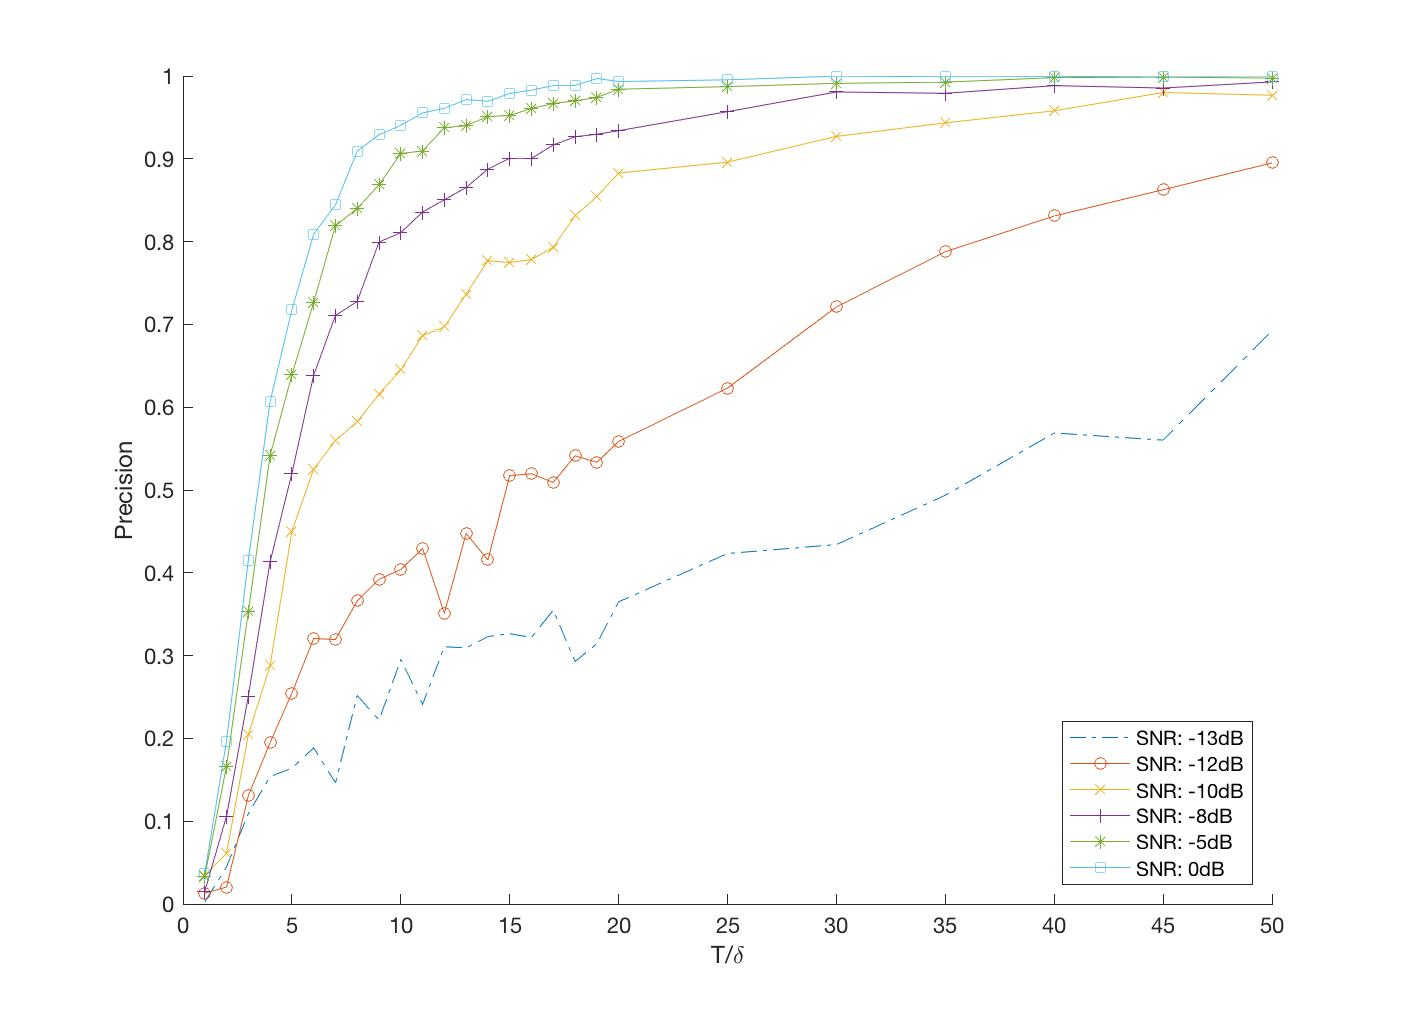
\includegraphics[width=0.8\textwidth]{test-align}
\caption{两路对齐算法测试结果\label{fig:test-align}}
\end{figure}

我们测试了信噪比为$-13dB$到$0dB$,$T/\delta$从0到50的情况,结果如图~\ref{fig:test-align}所示。图中可以看出,当信噪比低于$-12dB$时,对齐算法已经很难将语音完全对齐,这在本节开始时进行过讨论,因为信噪比过低,接收信号中的语音已经难以听清,自然难以实现时间对齐。而对齐的准确性随着$T/\delta$的增大而逐渐提高,在信噪比大于$-10dB$的情况下,$T/\delta$取到25以上就可以基本保证对齐的准确率在90\%以上,故可将$T/\delta$取为25。实际操作中,须首先估计或者测试原始相对延时$\delta$的大小,然后设定系统的$T$值大小。


\section{多路语音时间对齐} \label{section:align-multi}

在两路语音对齐算法的基础上,本节介绍一种实现多路语音时间对齐的算法。多路语音的时间对齐主要需要解决上小节算法给出的两两之间的相对延时可能存在不一致的问题,本文将该问题建模成图论问题,使用最小生成树算法进行优化选择,详述如下。

设收到有$K$路语音$(K\geq3$),分别为$y_1(t), y_2(t), ..., y_K(t)$,设指标集$I=\left\{i|i\in N^+, i\leq K\right\}$。首先使用~\ref{section:align2}节的方法我们可以估计出多路语音两两之间的相对延时$\delta_{ij}  (i,j\in I,i\neq j)$。

假设我们的估计不存在误差,且定义$\delta_{ii}=0,(i \in I)$,则

\begin{equation}\label{eq:delay-relations}
\delta_{ij}=\delta_{ik}+\delta_{jk}, \forall i,j,k \in I
\end{equation}

但是由于噪音的存在,延时的估计可能存在误差,所以两两之间的相对延时会存在不一致的情况,即公式~\ref{eq:delay-relations}并不恒成立。因而就需要从所有$K(K+1)/2$个相对延时中选取$K-1$个以确定一个统一的一致的,各路语音的相对延时。

一种最简单朴素的方法是以某一通道语音为基准,直接选取所有其他通道语音和该路语音的相对延时。例如以$y_1 (t)$为基准,选取$\delta_{1i}  (i \in I, i \neq 1)$作为统一标准确定各路语音的延时。但是这种方法得出的结果未必是最优的,如果 $y_1 (t)$ 受到的噪音污染较大,则很有可能得出的结果误差相当大。对此问题可以考虑使用后面介绍的语音质量客观评价方法来选取一路质量最优的语音作为参考基准。但是即便如此依然存在问题:如果选取的基准路语音$y_k (t)$和其他几路语音相对延时较大,而其他几路语音之间的相对延时较小,则估计的$y_k (t)$和其他几路语音的相对延时也会有较大误差,不如选取其他几路语音之间的相对延时加上$y_k (t)$和某一路语音的相对延时更好。

针对以上讨论的问题,以下介绍一种基于图论最小生成树算法来选取相对延时的方法。

我们的目标是要选取$K-1$个相对延时将所有K路语音关联起来,并使得选取的相对延时是估计准确性尽量高的。根据~\ref{section:align2}节的分析,对两路语音之间相对延时的估计的准确度可以通过互相关峰值的大小来反应,互相关的峰值越大,则准确性越高。以各路语音为节点构建一个全连通的有权无向图,各边的权值设为相连节点代表的两路语音之间互相关峰值的大小,则我们的目标可以描述为:选取$K-1$条边将$K$个节点连成一颗树,并使得$K-1$条边的权值和在所有的生成树中最大。即构造如下有权无向图
\begin{equation}
\begin{array}{l}
G(V,E), \\
V = I, \\
E = \left\{(i,j)|i, j\in I, i \neq j\right\}, \\
w(i,j)=\max⁡ \left\{ C_{ij}(\delta) \right\}
\end{array}
\end{equation}

问题即转化成求解图$G$的最大生成树,最大生成树和最小生成树可互相转化,直接对所有边权重求相反数即可。最小生成树是图论中非常经典的一个问题,有诸多相关的算法研究~\cite{bazlamaccci2001minimum}。

求解最小生成树问题的经典算法有Boruvka算法、Prim算法和Kruskal算法等。Boruvka算法是最古老的最小生成树算法,时间复杂度为$O(|E|log|V|)$;Prim算法和Kruskal算法是最常用的,也是最广为人知的两种最小生成树算法,时间复杂度分别为$O(|E|+|V|log|V|)$和$O(|E|log|E|)$。Yao~\cite{yao19750}在Boruvka算法基础上改进提出了一种更快速的算法,时间复杂度为$O(|E|loglog|V|)$。而Karger等人~\cite{karger1995randomized}提出的线性时间算法是目前最快的最小生成树算法。我们使用经典的Prim算法,如算法~\ref{alg:prim}所示。

\begin{algorithm}
    \caption{求解最小生成树的Prim算法}
    \label{alg:prim}
\begin{algorithmic}[1]
\INPUT
    \Statex 一个加权连通图,$G(V, E)$,其中V为顶点集合,E为边集合
\OUTPUT
    \Statex 最小生成树$T(V_T, E_T)$,其中$V_T = V$是最小生成树的顶点集合,$E_T \in E$是最小生成树的边集合
\State 初始化$V_T = {x}$,其中$x$为集合$V$中的任一顶点,$E_T = {}$,为空
\State $i=l-1, j=r+1, k=l$
\While { $V_T \neq V$; }
    \State 在集合$E$中选取权值最小的边$<u, v>$,其中$u \in V_T, v \not\in V_T$;
    \State 将边$<u, v>$加入集合$E_T$,顶点$v$加入集合$V_T$
\EndWhile
\end{algorithmic}
\end{algorithm}

得到最大生成树后,生成树上对应的边即代表应该选取的相对延迟估计,在这$K-1$个相对延迟的基础上,利用式~\ref{eq:delay-relations}即可求出各路信号相对$y_1 (t)$的延迟$\delta_{i1},(i \in I)$,其中$\delta_{11}=0$。随后对各路信号进行对齐和平移,得到时间对齐后的信号:
\begin{equation}
y_i^* (t)=y_i (t+\delta_{i1}-\min_{j\in I}\delta_{j1})
\end{equation}

类似两路对齐算法,我们对多路对齐算法也进行了相应的测试。我们生成了具有不同延时的5路语音信号,并给他们添加不同能量大小的高斯噪音以测试不同信噪比的情况。生成的5路语音延时如表~\ref{tab:delays}所示。为了与两路语音对齐做比较,我们特意设置通路1和通路5之间的相对延时为10ms,与两路语音对齐测试一致。

\begin{table}
\centering
\caption{测试用各路语音延时}
\label{tab:delays}
\begin{tabular}{ccc}
\toprule[1.5pt]
通路编号 & 相对通路1的延时$\delta_{i1}$ \\ \midrule[1pt]
1 & 0ms \\
2 & -3ms \\
3 & 2ms \\
4 & 6ms \\
5 & 10ms \\ \bottomrule[1.5pt]
\end{tabular}
\end{table}

\begin{figure}
\centering
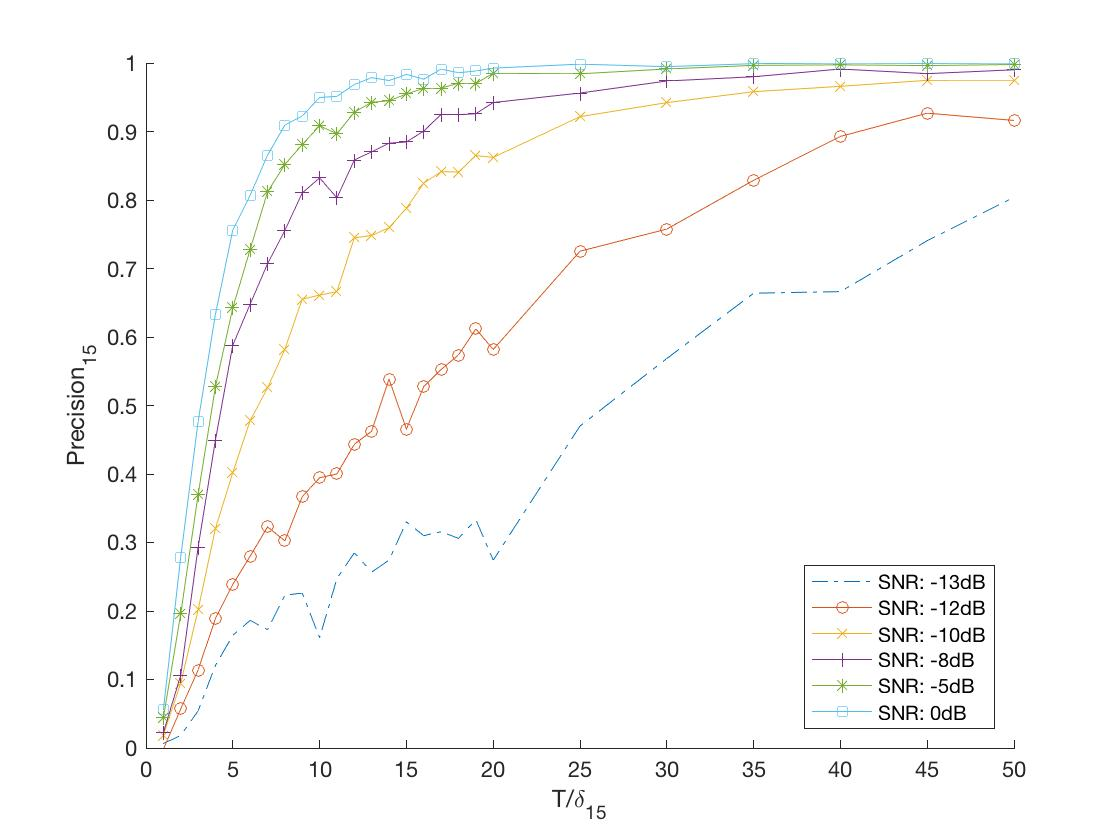
\includegraphics[width=0.8\textwidth]{test-align-multi}
\caption{多路对齐算法测试结果\label{fig:test-align-multi}}
\end{figure}

\begin{figure}
\centering
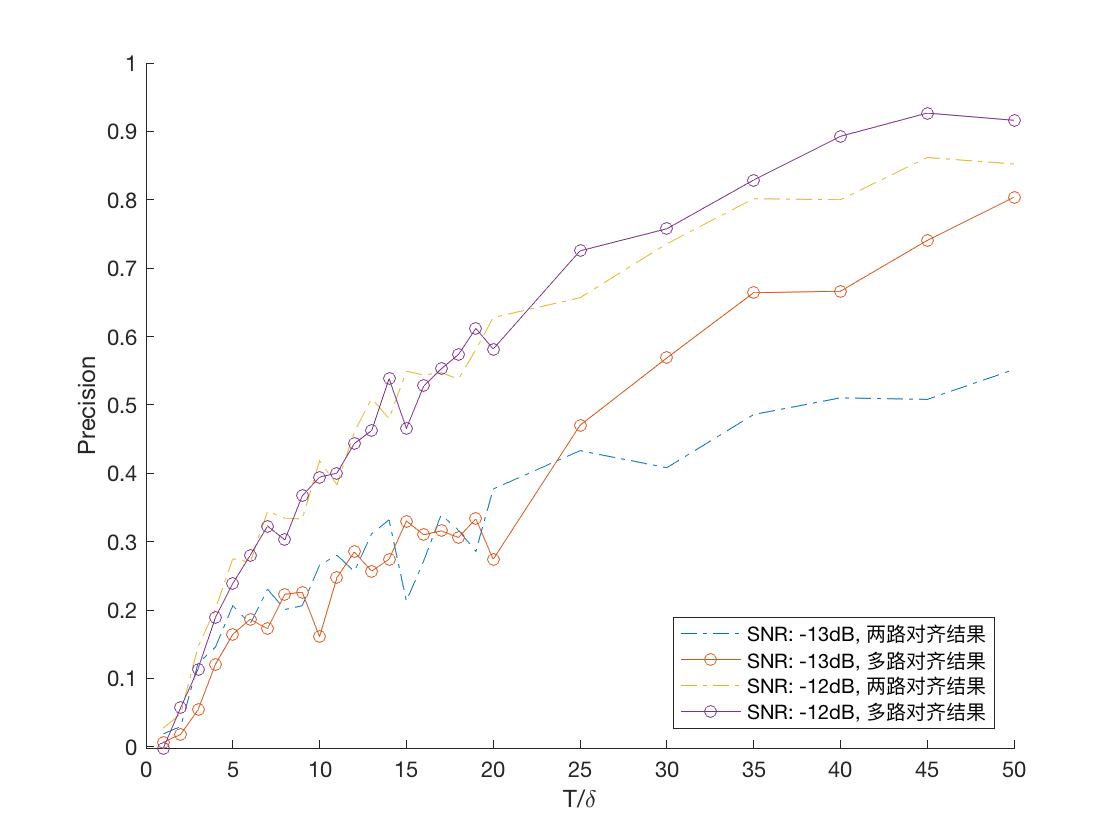
\includegraphics[width=0.8\textwidth]{compare-align}
\caption{多路对齐算法与两路对齐算法比较\label{fig:compare-align}}
\end{figure}

我们测试信噪比从$-13dB$到$0dB$,$T/\delta_{15}$从0到50的情况,分析多路对齐算法对通路1和通路5对齐结果的准确性,每组实验进行1000次取平均,结果如图~\ref{fig:test-align-multi}所示。可以看到和两路语音对齐一样,对于信噪比在$12dB$以上的情况,$T/\delta_{15} > 25$就可以基本保证90\%以上的对齐准确率。

而且,由于我们使用最小生成树策略在5路信号之间选择了更可信的4对相对延时时间构建了整体的相对延时,使得在低信噪比的情况下,多路对齐的结果比直接两路对齐的效果更好。如图~\ref{fig:compare-align}所示,我们比较了信噪比为$-13dB$和$-12dB$情况下,直接两路对齐和多路对齐的结果,其中多路对齐选择1路和5路的对齐准确率,这两路信号的相对延时为10ms,与两路对齐测试中一致。由于利用了另外三路信号的信息,可以看到多路对齐的结果要明显由于直接两路对齐的结果,可见我们多路对齐算法的策略起到了很好的作用。

\section{实时多路对齐算法} \label{section:realtime-align}

实际应用中,往往要求对多路语音信号进行实时处理。在~\ref{section:align-multi}节基础上,本节介绍一种对于多路语音信号流进行实时对齐的算法。

在实时的信号处理中,缓冲队列是非常常见的结构,本文采用多级缓冲队列的形式实现实时的多路语音对齐。第一级缓冲队列接收各路信号的输入,对于每一路语音使用一个缓冲队列存储最近一段时间的信号,新到达的信号从队尾加入队列,通过对齐算法计算各路语音的相对延时从而控制各路信号出队列的时间,也即进入第二级缓冲队列的时间,使得第二级缓冲队列中的各路信号是时间对齐的,可用于后续的计算和处理。

\begin{figure}
\centering
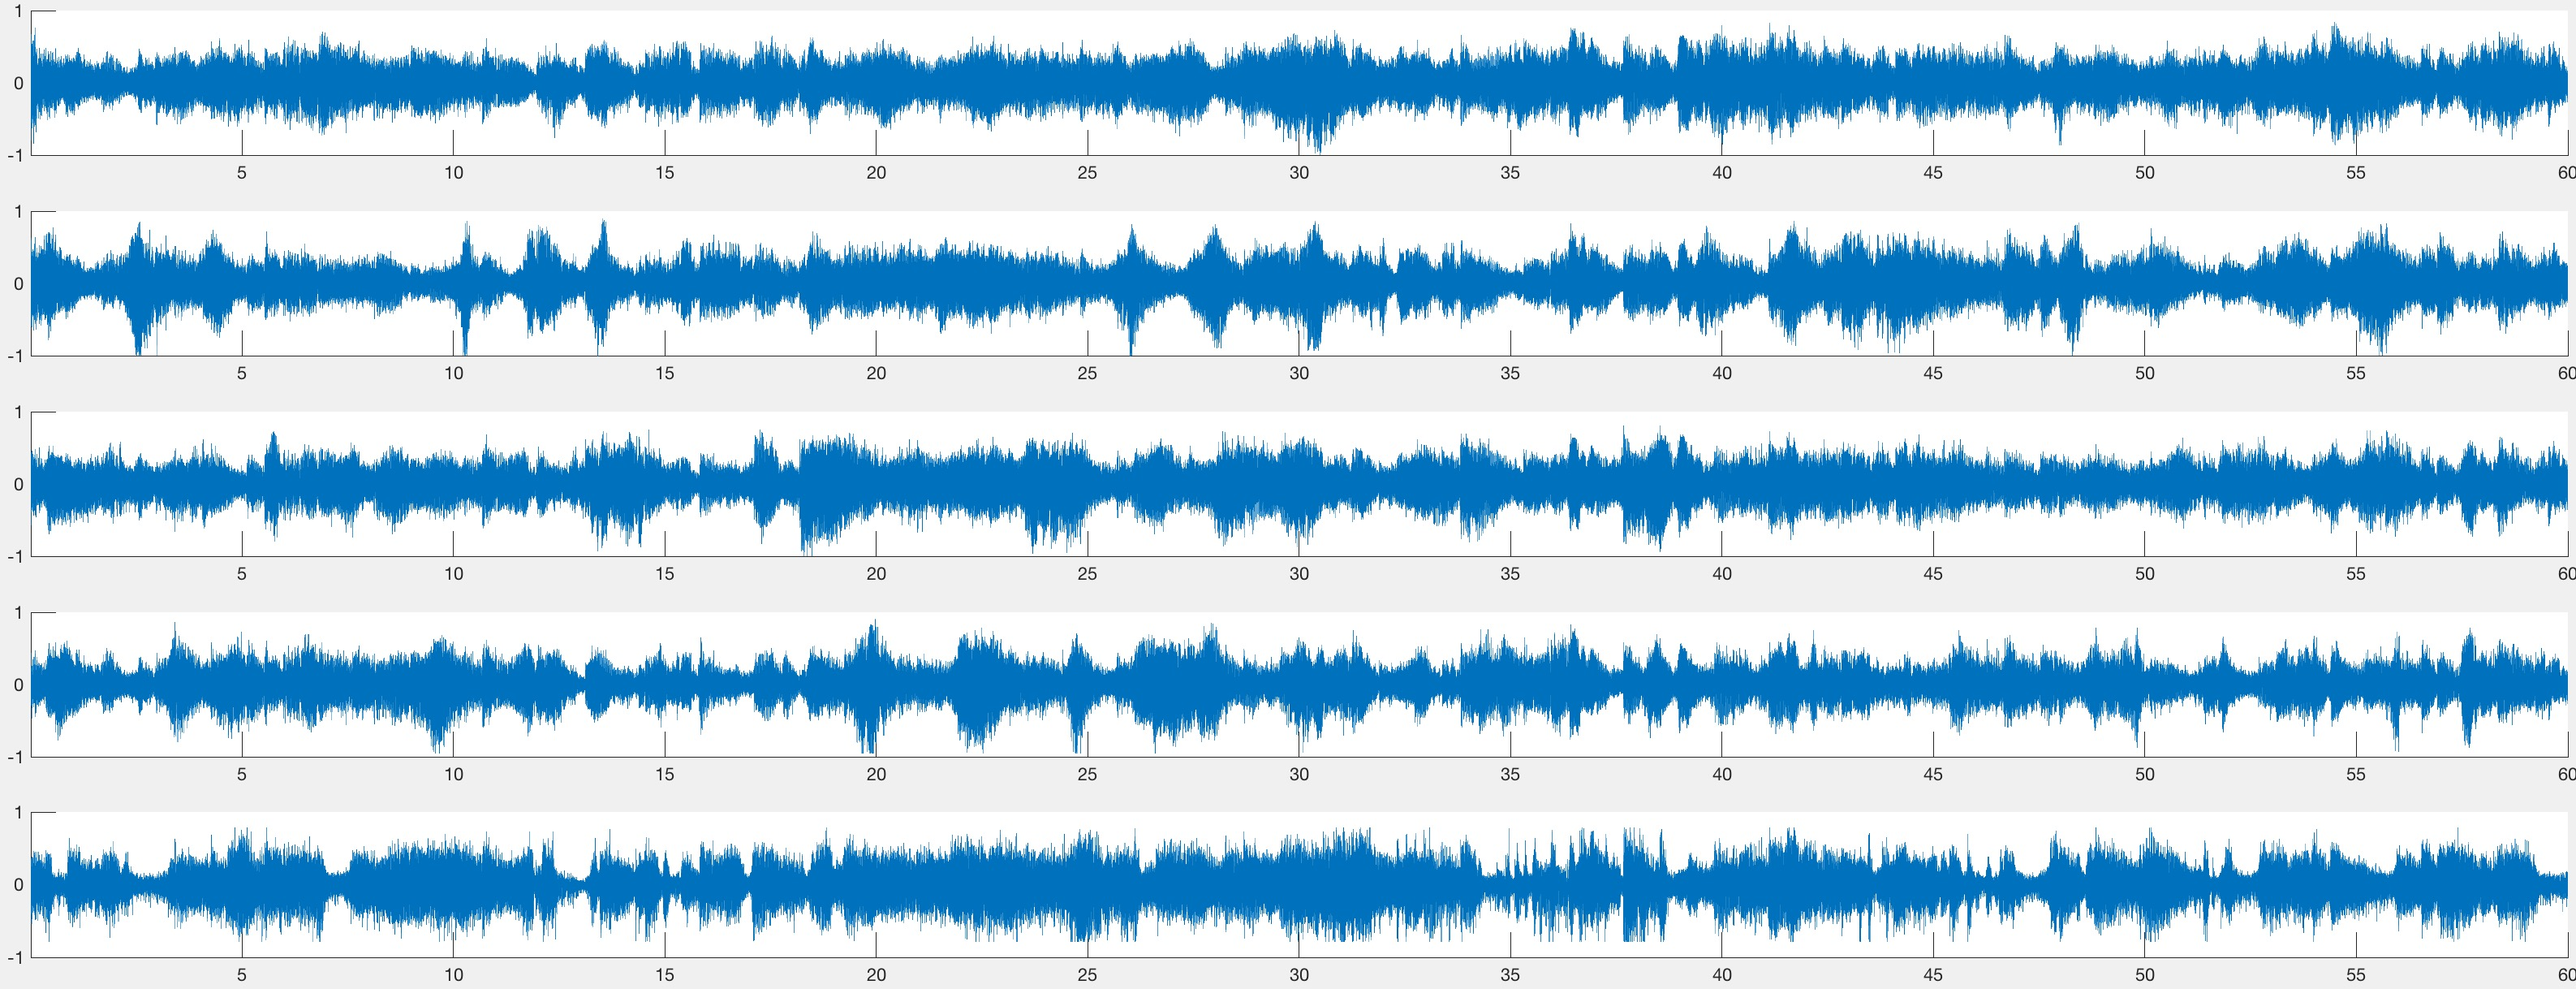
\includegraphics[width=0.8\textwidth]{multi-align}
\caption{实时对齐算法示意\label{fig:multi-align}}
\end{figure}

为便于理解,可以想象语音信号是固定的队列,而一级缓冲队列则是在移动的队首和队尾指针。如图~\ref{fig:multi-align}所示,将语音信号想象成一个无限长的队列,然后有一个队首指针和队尾指针,两个指针之间的部分即使算法目前实际缓存的语音信号部分。由于随着时间推移不断接收到新的信号,所以队尾指针会随着时间以固定速率后移,而队首指针则是在算法控制下后移以调整延时,最终稳定时,队首和队尾的指针均匀速后移,各路信号缓存的长度不同,队首指针处的信号是时间上对齐的,各个一级缓冲队列的队列长度则因为信号延时不同而不同。

算法一开始首先保证各路信号均缓存了时间长度为的数据。随后使用~\ref{section:align-multi}节中的算法可以得出各路信号相对第一路信号的延迟$\delta_{i1}, i \in I$,可能为负值,找到最大的延时,记为$\delta_{k1} = \max \delta_{i1}$,则为了保证队首指针时间对齐,第$i$路信号的队首指针应暂停$\delta_{k1}-\delta_{i1}$时间不移动。这相当于第$i$路信号的延迟增加了$\delta_{k1}-\delta_{i1}$,于是各路信号的队首均对齐到了路信号。之后每0.1秒执行一次上述步骤进行对齐调整。

进一步,为了保证算法的稳定性,降低执行过程中对于相对延时突发的错误估计造成的影响,可以设置一个调整步长$0<\alpha<1$,各路队首指针暂停时间修改为$\alpha(\delta_{k1}-\delta_{i1})$。$\alpha$越大则越快收敛到对齐状态,但是越不稳定;相反越小则收敛速度越慢,但是越稳定。可以根据情况设定$\alpha$的取值。

另外,此方法永远在增加信号的延迟,会导致合路信号的延迟越来越大,可以做如下改进:每次对齐调整完成后,如果最短的缓存队列长度为超过了$T$,则所有路信号的队首指针同时向后调整使得最短的缓存队列长度缩短为$T$。这样,合路信号的延迟永远为延迟最大的一路信号的延迟加上$T$。

最终的算法流程参见算法~\ref{alg:live-align}。

\begin{algorithm}
    \caption{多路语音实时对齐算法}
    \label{alg:live-align}
\begin{algorithmic}[1]
\INPUT
    \Statex 实时推送的多路语音信号
\OUTPUT
    \Statex 实时输出时间对齐的多路语音信号
\State 初始化多路语音的缓冲队列$Q_i, i\in I$,接收到的各路语音会定时进入各个队列的队尾
\State 等待各路语音的缓冲队列长度超过$T$
\State 初始化各路语音信号的时间调节变量$D_i$全部为0
\While { true; }
    \For { $i \in I$ }
        \If { $D_i = 0$ }
            \State 语音缓冲队列$Q_i$队首出队列并且输出
        \Else
            \State $Q_i = Q_i - 1$
        \EndIf
    \EndFor
    \If { 所有的$Q_i$的长度均超过$T$ }
        \State 所有语音缓冲队列队首出队列并且输出
    \EndIf
    \If { 距上一次计算相对延迟已达到0.1秒或尚未计算相对延迟 }
        \State 使用~\ref{section:align-multi}节描述的算法计算各路语音的相对延时$\delta_{ij}$
        \State 在$\delta_{i1}$中找到最大值$\delta_{k1}$
        \For { $i \in I$ }
            \State $D_i = D_i + \alpha(\delta_{k1}-\delta_{ki})$
        \EndFor
    \EndIf
    \State 休眠一个采样时间
\EndWhile
\end{algorithmic}
\end{algorithm}

\section{选路策略及系统设计}

本节介绍短波语音信号的选路策略以及选路系统的设计。由于各路信号的强度和背景噪音不同,如果直接对各段时间内的信号,总是切换到质量评分最高的一路信号,可能出现信号切换过于频繁,导致听起来连贯的问题,反而影响合路信号的质量。以下几项策略保证了合路信号在选择尽量优质量的语音通路的同时,提高合路语音的自然度。

\begin{enumerate}
    \item 需要对各路语音的功率进行归一化处理,可以使用各路语音的均值功率作为参考,将各路语音信号放大或缩小从而统一功率。
    \item 为防止意外状况导致的错误评分带来的抖动,对各路语音的实时评分经过一个低通滤波作为选路参考的分值。
    \item 为了避免过度频繁的切换语音通路,设定一个适当大小的阈值,只有当新的最优通路的评分超过当前选择通路的评分达到一定阈值,才切换至新的最优通路。否则依然保持原来选择的通路。 
    \item 在通路切换时,采用线性渐变的过度来平滑切换的过程。
\end{enumerate}

\begin{figure}
\centering
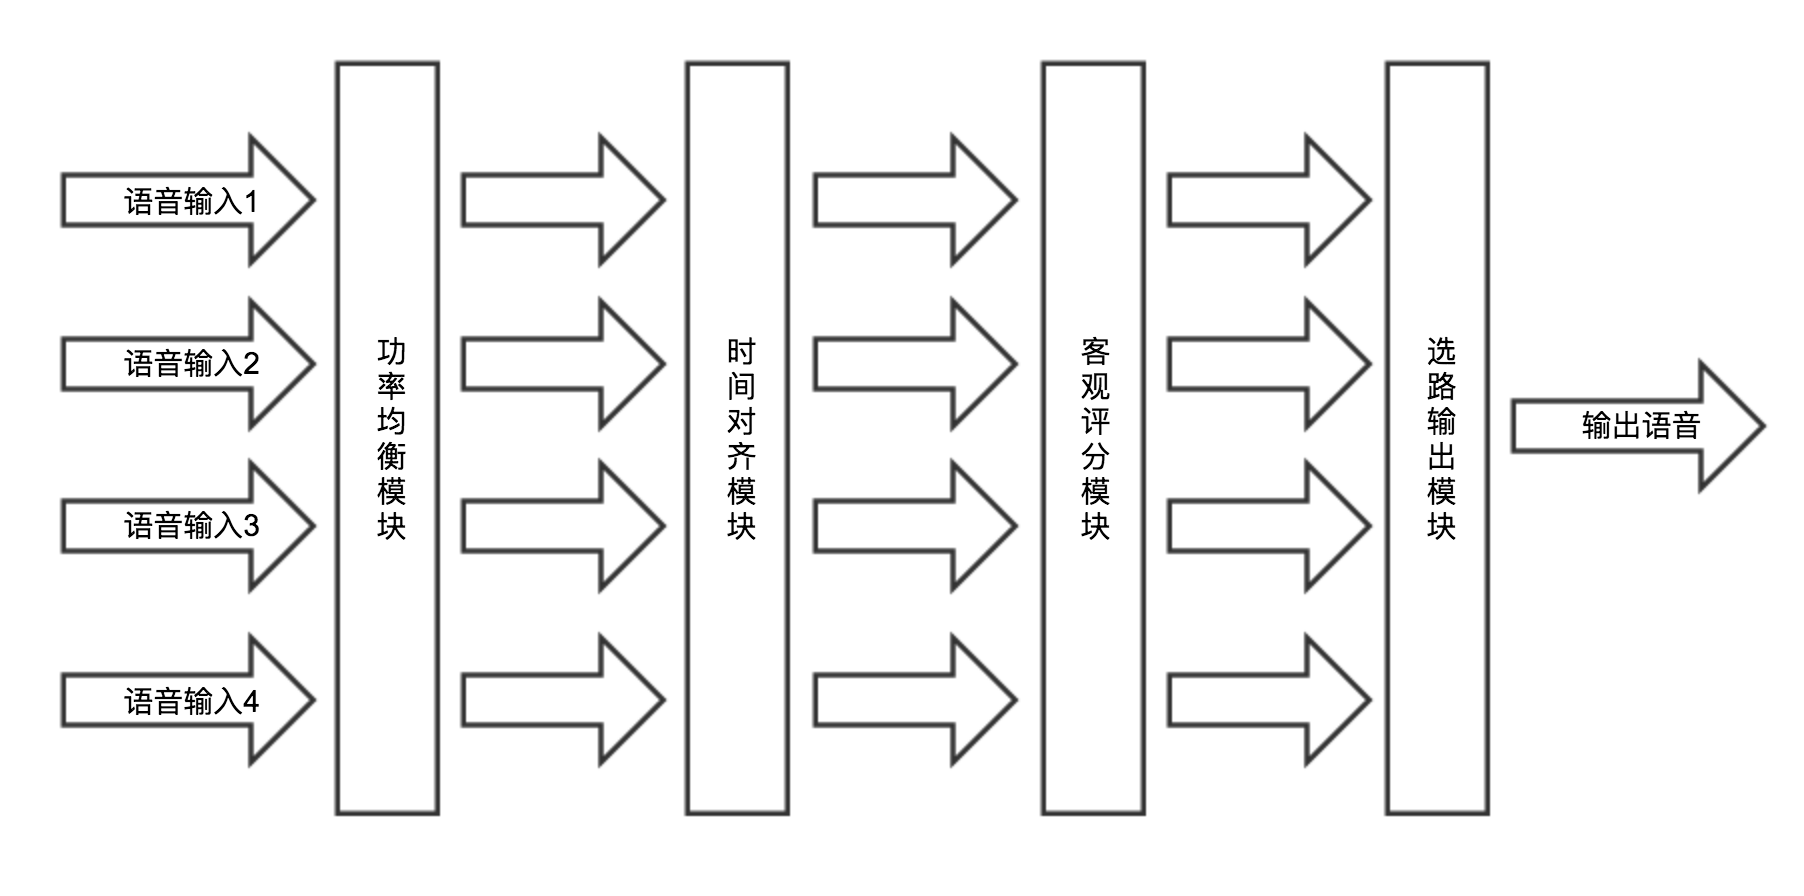
\includegraphics[width=0.8\textwidth]{switching-sys}
\caption{选路系统结构\label{fig:switching-sys}}
\end{figure}

如图~\ref{fig:switching-sys}所示,选路系统分为“功率均衡模块”、“时间对齐模块”、“客观评分模块”、“选路输出模块”这四个模块,分别实现上述几项策略。

功率均衡模块负责均衡各路语音信号的功率,具体步骤如下:统计每一路输入最近1s时间内的信号功率$P_i, i \in I$,将其经过一个低通滤波器,得到滤波后的平均信号功率$\bar{P_i}$,据此可利用式~\ref{eq:power-gain}计算各路的信号增益$Gain_i$,各路信号分别乘上对应增益实现各路信号的功率均衡。
\begin{equation}\label{eq:power-gain}
Gain_i = \sqrt{\frac {K\bar{P_i}} {\sum_{k \in I}{\bar{P_k}}} }
\end{equation}

时间对齐模块负责各路语音信号的时间对齐,使用~\ref{section:realtime-align}节介绍的算法实现。

客观评分模块对每一路最近1s内的信号使用第~\ref{chapter:algorithms}章介绍的算法进行客观评分,然后再通过低通滤波器得到去除抖动后的质量评分$\bar{S_i}, i \in I$。

选路输出模块负责选路切换,设定切换阈值$T_{switch}$,若当前输出为$i$路语音,切换到第$j$路语音的条件为:
\begin{equation}
\begin{array}{l}
\bar{S_j} = \max\limits_{k \in I} \bar{S_k} \\
\bar{S_j} - \bar{S_i} > T_{switch}
\end{array}
\end{equation}

在发生切换时,切换模块自动完成线性平滑过度,设定切换时长为$\Delta$,则切换阶段输出语音可表示为:
\begin{equation}
y_{out}(t) = \frac{ty_j(t)+(\Delta-t)y_i(t)}{\Delta}
\end{equation}

\section{小结}

本章主要介绍了短波语音自动选路系统。首先介绍了关键的多路语音时间对齐算法,包括基于互相关的两路语音时间对齐算法、基于最小生成树的多路语音时间对齐算法以及使用缓冲队列实现的实时对齐算法。然后介绍了自动选路系统的设计,包括功率均衡模块、时间对齐模块、客观评分模块和选路切换模块。该系统通过自动客观评分切换选择质量最优的一路信号,并且利用时间对齐算法、功率均衡策略、平滑滤波以及阈值切换策略等保证了输出语音的连贯性。
